% 2011 年福建卷理科第 20 题：四棱锥 P-ABCD，PA⊥底面，AB⊥AD。
% 来源 PDF：普通高考/2011/2011福建理.pdf，SHA-256 1a36c388b64669b29d16fe359efb087d96026059df01d26759f8bb5dd48342f1。
% 原页：第 2 页第 2 栏上部，书页码 660。示意。
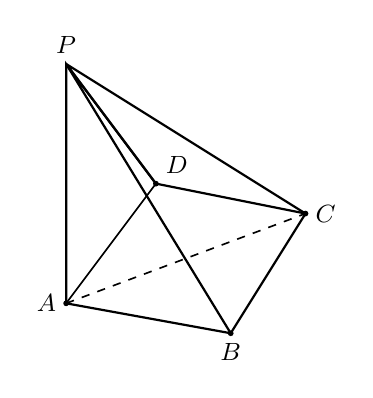
\begin{tikzpicture}[>=stealth, semithick, font=\small, scale=0.95]
  \coordinate (A) at (0,0);
  \coordinate (B) at (2.2,-0.4);
  \coordinate (D) at (1.2,1.6);
  \coordinate (C) at (3.2,1.2);
  \coordinate (P) at (0,3.2);
  \draw[thick] (P)--(A)--(B)--(C)--(D)--cycle;
  \draw[thick] (P)--(B) (P)--(C) (P)--(D);
  \draw[dashed] (A)--(C);
  \draw (A)--(D);
  \fill (A) circle (1.1pt) node[left] {$A$};
  \fill (B) circle (1.1pt) node[below] {$B$};
  \fill (C) circle (1.1pt) node[right] {$C$};
  \fill (D) circle (1.1pt) node[above right] {$D$};
  \node[above] at (P) {$P$};
\end{tikzpicture}
